\documentclass[../../main.tex]{subfiles}

\graphicspath{{../../image/}{../../figure/}}

\begin{document}

\section{信息论}\label{section:ch02-信息论}

概率论为另一个重要的框架——信息论（information theory）提供了基础。它量化了数据集中存在的信息，并在机器学习中扮演着重要角色。这里简要介绍一些本书后面需要用到的信息论中的关键元素，包括熵的重要概念及其各种变体。关于信息论的更全面介绍及其与机器学习的联系，参见 MacKay（2003）。

\subsection{熵}\label{subsection:ch02-熵}

考虑一个离散随机变量 $x$，我们想知道当观察到这个变量的某个特定值时能获得多少信息。信息量可以视为我们在得知 $x$ 的具体值时的“惊讶程度”。如果我们被告知一个极不可能发生的事件刚刚发生了，那么我们接受到的信息将多于某个极有可能发生的事件刚刚发生的信息。如果我们知道某个事件确定会发生，那么我们不会接收到任何信息。信息内容的度量将依赖于概率分布 $p(x)$。我们需要寻找一个量 $h(x)$，它是概率 $p(x)$ 的单调函数，并且表达了信息的内容。注意，如果两个事件 $x$ 和 $y$ 是无关的，那么观察它们所获得的信息增益应该是分别观察它们所获得的信息增益之和，即 $h(x,y)=h(x)+h(y)$。两个无关的事件是统计独立的，所以 $p(x,y)=p(x)p(y)$。由这两个关系可知 $h(x)$ 必须由 $p(x)$ 的对数给出（见\cref{exercise:ch02-21}），所以有

\begin{align}
  h(x) = -\log_2 p(x)
  \label{align:ch02-信息量}
\end{align}

\begin{definition}[信息量]\label{definition:ch02-信息量}
称由\eqref{align:ch02-信息量}定义的量 $h(x)$ 为事件 $x$ 发生的\textbf{信息量}。它以 2 为底的对数，单位称为\textbf{比特}（bit，即“二进制位”）；若改用自然对数，单位称为\textbf{纳特}（nat）。
\end{definition}

% SUPPLEMENT: parent=definition:ch02-信息量; kind=motivation; location=紧随其后的 remark（重构新增）
\begin{remark}（重构新增）
定义中的负号是必要的：$0<p(x)\leqslant1$ 时 $\log_2p(x)\leqslant0$，加负号后 $h(x)\geqslant0$，符合“信息量非负”的直觉。同时，$p(x)$ 越小 $h(x)$ 越大，恰好刻画了“越意外、信息越多”。

底数的选取只影响单位而不影响比较：以 2 为底得比特，以 $e$ 为底得纳特，二者相差常数因子 $\ln2$，即 $1$ 纳特 $\approx1.44$ 比特。这一自由度在\eqref{align:ch02-信息量}中体现为“对数的底数选取是任意的”，但一旦选定就必须在整节中保持一致。
\end{remark}

其中负号确保了信息是正的或为零。注意低概率事件 $x$ 对应于高信息内容。对数的底数选取是任意的，此刻我们采用信息论中的惯例，即以 2 为底数。在这种情况下，我们可以看到 $h(x)$ 的单位是比特（“二进制位”）。

现在假设发送者希望向接收者传输一个随机变量的值。他们在这个过程中传输的平均信息量是通过对\eqref{align:ch02-信息量}关于分布 $p(x)$ 取期望得到的，由下式给出：

\begin{align}
  H[x] = -\sum_{x} p(x)\log_2 p(x)
  \label{align:ch02-离散熵}
\end{align}

\begin{proposition}[独立事件的信息量可加]\label{proposition:ch02-信息量可加}
设事件 $x$ 与 $y$ 统计独立，则 $h(x,y)=h(x)+h(y)$。
\end{proposition}

\begin{proof}
由独立性 $p(x,y)=p(x)p(y)$，代入\eqref{align:ch02-信息量}并对数化积为和：
\begin{align*}
  h(x,y) = -\log_2\big(p(x)p(y)\big) = -\log_2p(x) - \log_2p(y) = h(x)+h(y) .
\end{align*}
\end{proof}

% SUPPLEMENT: parent=proposition:ch02-信息量可加; kind=motivation; location=紧随其后的 remark（重构新增）
\begin{remark}（重构新增）
可加性是对“信息量”这一概念的基本要求：两个互不相关的事件所提供的总信息应当等于各自信息之和，否则“信息”就不能像长度、时间那样累加，编码长度的讨论也失去意义。

这条性质与\eqref{align:ch02-信息量}的对数形式互为因果：正因为 $\log$ 把乘积变成和，定义才能同时满足“单调”与“独立可加”。\cref{exercise:ch02-21}进一步证明，在适当的连续性假设下，$-\log_2p$ 是唯一满足这两条要求的函数形式。
\end{remark}

这个重要的量称为随机变量 $x$ 的熵（entropy）。注意 $\lim_{\varepsilon\to0}(\varepsilon\ln\varepsilon)=0$，所以当遇到 $x$ 在某个取值下使 $p(x)=0$ 时，令 $p(x)\ln p(x)=0$。

\begin{definition}[熵]\label{definition:ch02-熵}
称由\eqref{align:ch02-离散熵}定义的量 $H[x]$ 为离散随机变量 $x$ 的\textbf{熵}（entropy），它是信息量 $h(x)$ 在分布 $p(x)$ 下的期望，即对 $x$ 的不确定性的度量。
\end{definition}

% SUPPLEMENT: parent=definition:ch02-熵; kind=motivation; location=紧随其后的 remark（重构新增）
\begin{remark}（重构新增）
熵是“平均惊讶程度”：它把每个取值的惊讶程度 $h(x)$ 按该取值出现的概率加权平均。因此熵只依赖分布的形状，不依赖取值的具体标签——把 $x$ 的取值重新命名不会改变熵，这一点与期望不同。

\eqref{align:ch02-离散熵}中的约定 $0\ln0=0$ 不可省：否则 $p(x)=0$ 的取值会使求和无定义。该约定的合法性来自 $\lim_{\varepsilon\to0}\varepsilon\ln\varepsilon=0$，它保证了熵对分布是连续的——概率的微小改变只会引起熵的微小改变。
\end{remark}

到目前为止，我们已经启发式地给出了信息［\eqref{align:ch02-信息量}］和相应的熵［\eqref{align:ch02-离散熵}］的定义。这些定义确实具有一些有用的性质。考虑一个有 $8$ 个可能状态的随机变量 $x$。为了将 $x$ 的值传输给接收者，我们需要传输一条长度为 $3$ 比特的消息。注意，这个变量的熵由下式给出：

\begin{align}
  H[x] = -8\times\frac{1}{8}\log_2\frac{1}{8} = 3 \text{（比特）}
  \label{align:ch02-八状态熵}
\end{align}

举个例子（Cover and Thomas, 1991），一个变量有 $8$ 个可能的状态 $\{a,b,c,d,e,f,g,h\}$，各自的概率分别为 $\left(\frac{1}{2},\frac{1}{4},\frac{1}{8},\frac{1}{16},\frac{1}{64},\frac{1}{64},\frac{1}{64},\frac{1}{64}\right)$。这种情况下的熵由下式给出：

\begin{align}
  H[x] = -\frac{1}{2}\log_2\frac{1}{2} - \frac{1}{4}\log_2\frac{1}{4} - \frac{1}{8}\log_2\frac{1}{8} - \frac{1}{16}\log_2\frac{1}{16} - 4\times\frac{1}{64}\log_2\frac{1}{64} = 2 \text{（比特）}
  \label{align:ch02-非均匀熵}
\end{align}

可以看出，非均匀分布的熵小于均匀分布的熵，稍后在讨论熵的混乱度时，我们将对此有所了解。考虑如何将变量的状态传输给接收者。我们既可以像之前那样使用一个 $3$ 比特的数字，也可以使用较短编码来表示较大可能发生的事件，或用较长编码表示较小可能发生的事件，从而利用非均匀分布的特点，实现较短的平均编码长度。这一目的可以通过使用以下一组代码字符串表示状态 $\{a,b,c,d,e,f,g,h\}$ 来实现，例如 $0$、$10$、$110$、$1110$、$111100$、$111101$、$111110$ 和 $111111$。必须传输的代码的平均长度为

\begin{align}
  \text{代码平均长度} = \frac{1}{2}\times1 + \frac{1}{4}\times2 + \frac{1}{8}\times3 + \frac{1}{16}\times4 + 4\times\frac{1}{64}\times6 = 2 \text{（比特）}
  \label{align:ch02-平均编码长度}
\end{align}

这与随机变量的熵相同。注意，我们已经不能使用再短的代码字符串了，因为必须保证由这些状态编码拼接起来的序列能被无歧义地分解为每个状态。例如，$11001110$ 只能唯一地解码为状态序列 $c,a,d$。熵和最短编码长度之间的这种关系具有一般性。

\begin{example}[ 熵与平均编码长度]\label{example:ch02-熵与编码}
比较两个 $8$ 状态随机变量。

（1）等概率情形：$p(x_k)=1/8$，由\eqref{align:ch02-八状态熵}，$H[x]=3$ 比特，恰等于用长度 $3$ 的二进制串逐一编码所需的比特数。

（2）非均匀情形：概率为 $(1/2,1/4,1/8,1/16,1/64,1/64,1/64,1/64)$，由\eqref{align:ch02-非均匀熵}，$H[x]=2$ 比特，小于等概率情形的 $3$ 比特；而\eqref{align:ch02-平均编码长度}给出的前缀码 $0,10,110,1110,111100,111101,111110,111111$ 的平均长度也恰为 $2$ 比特。

（3）该前缀码可以唯一解码：任一码字都不是另一码字的前缀，故拼接后的串从左向右读时，遇到第一个完整码字即可分割。例如 $11001110\to110|0|1110\to c,a,d$。
\end{example}

\begin{theorem}[无噪编码定理]\label{theorem:ch02-无噪编码定理}
设离散随机变量 $x$ 取值 $x_1,\cdots,x_K$，概率为 $p_1,\cdots,p_K$，$H[x]=-\sum_k p_k\log_2p_k$。则对 $x$ 的任一前缀码，其平均码长 $L=\sum_k p_k l_k$ 满足 $L\geqslant H[x]$；且存在前缀码使 $L<H[x]+1$。
\end{theorem}

\begin{proof}
先证下界。设码字长度为 $l_1,\cdots,l_K$。前缀码的 Kraft 不等式成立：$\sum_{k=1}^{K}2^{-l_k}\leqslant1$（前缀码对应一棵二叉树的叶，第 $k$ 个叶可分配长度 $2^{-l_k}$ 的互不重叠的单位区间，故这些长度之和不超过 $1$）。记 $q_k=2^{-l_k}$、$K_0=\sum_kq_k\leqslant1$，则由对数求和不等式（见下面的说明）取 $a_k=p_k$、$b_k=q_k$，
\begin{align*}
  L - H[x] = \sum_{k=1}^{K}p_k\log_2\frac{p_k}{q_k}
  \geqslant \left(\sum_{k=1}^{K}p_k\right)\log_2\frac{\sum_{k=1}^{K}p_k}{\sum_{k=1}^{K}q_k}
  = \log_2\frac{1}{K_0} \geqslant 0 ,
\end{align*}
故 $L\geqslant H[x]$。这里用到的对数求和不等式为：对 $a_k,b_k>0$，
\begin{align*}
  \sum_k a_k\ln\frac{a_k}{b_k} \geqslant \Big(\sum_k a_k\Big)\ln\frac{\sum_k a_k}{\sum_k b_k} ,
\end{align*}
它由初等不等式 $\ln t\geqslant1-1/t\ (t>0)$ 得到：令 $A=\sum_ka_k$、$B=\sum_kb_k$，则
\begin{align*}
  \sum_k\frac{a_k}{A}\ln\frac{a_kB}{b_kA}
  \geqslant \sum_k\frac{a_k}{A}\left(1-\frac{b_kA}{a_kB}\right)
  = \sum_k\frac{a_k}{A} - \sum_k\frac{b_k}{B} = 1-1 = 0 .
\end{align*}

再证上界：取 $l_k=\lceil-\log_2p_k\rceil$，则 $2^{-l_k}\leqslant p_k$，从而 $\sum_k2^{-l_k}\leqslant\sum_kp_k=1$，由 Kraft 不等式的逆定理存在以这些长度为码长的前缀码；而 $l_k<-\log_2p_k+1$，故 $L=\sum_kp_kl_k<H[x]+1$。
\end{proof}

% SUPPLEMENT: parent=theorem:ch02-无噪编码定理; kind=motivation; location=紧随其后的 remark（重构新增）
\begin{remark}（重构新增）
定理把“熵”从一个启发式的量提升为一个可操作的下界：任何无损压缩方案的平均码长都不可能低于熵，而熵加 $1$ 比特之内总能达到。这也解释了\eqref{align:ch02-非均匀熵}与\eqref{align:ch02-平均编码长度}数值相同并非巧合。

证明的关键是 Kraft 不等式，它把“前缀码存在”转化为“一组长度满足 $\sum2^{-l_k}\leqslant1$”。条件“前缀码”不可省：若允许非前缀码，则可能出现歧义解码（例如把 $0$ 与 $01$ 同时作为码字），此时下界不再成立。定理是 Shannon（1948）的经典结果，本书只引用其结论。
\end{remark}

从现在开始，我们将改用自然对数来定义熵，以便与本书其他部分的观点联系起来。在这种情况下，熵以纳特（nat）（源自“自然对数”）而不是比特为单位度量，$1$ 纳特约 $1.44$ 比特。

\subsection{物理学视角}\label{subsection:ch02-物理学视角}

我们已经以明确随机变量特定状态所需的平均信息量的形式介绍了熵的概念。实际上，熵的概念在物理学中有着更早的起源。熵在平衡热力学的背景下被引入，后续随着统计力学的发展，熵被赋予更深层次的解释，即作为无序程度的度量指标。我们也可以从这种视角来理解熵。假设有 $N$ 个相同的物品要被分配到一组箱子中，其中第 $i$ 个箱子中有 $n_i$ 个物品。有多少种不同的方式可以将物品分配到箱子中。选择第一个物品有 $N$ 种方式，选择第二个物品有 $(N-1)$ 种方式，以此类推，总共有 $N!$（读作“$N$ 的阶乘”）种方式将所有 $N$ 个物品分配到箱子中，其中 $N!$ 表示乘积 $N\times(N-1)\times\cdots\times2\times1$。然而，我们无须区分每个箱子内的物品是否重新排列。在第 $i$ 个箱子中重新排列物品的方式有 $n_i!$ 种，因此将 $N$ 个物品分配到箱子中的总方式数由下式给出：

\begin{align}
  W = \frac{N!}{\prod_i n_i!}
  \label{align:ch02-多重数}
\end{align}

$W$ 表示多重数（multiplicity）。然后，熵被定义为多重数的对数并通过常数因子 $1/N$ 变换尺度，所以有

\begin{align}
  H = \frac{1}{N}\ln W = \frac{1}{N}\ln N! - \frac{1}{N}\sum_i\ln n_i!
  \label{align:ch02-熵与多重数}
\end{align}

考虑极限 $N\to\infty$，其中分数 $n_i/N$ 保持固定，并应用 Stirling 公式

\begin{align}
  \ln N! \approx N\ln N - N
  \label{align:ch02-Stirling}
\end{align}

可以得到

\begin{align}
  H = -\lim_{N\to\infty}\sum_i\frac{n_i}{N}\ln\frac{n_i}{N} = -\sum_i p_i\ln p_i
  \label{align:ch02-熵与概率}
\end{align}

\begin{definition}[多重数、微观状态与宏观状态]\label{definition:ch02-多重数}
设 $N$ 个物品被分配到若干箱子中，第 $i$ 个箱子中有 $n_i$ 个物品。称\eqref{align:ch02-多重数}给出的 $W$ 为该分配的\textbf{多重数}（multiplicity）。在物理学中，物品到箱子的具体分配称为\textbf{微观状态}（microstate），而仅由各箱物品数（用比例 $n_i/N$ 表示）决定的分配方式称为\textbf{宏观状态}（macrostate）；$W$ 表达给定宏观状态所包含的微观状态数量，也称该宏观状态的\textbf{权重}（weight）。
\end{definition}

% SUPPLEMENT: parent=definition:ch02-多重数; kind=motivation; location=紧随其后的 remark（重构新增）
\begin{remark}（重构新增）
引入多重数的动机是把“熵”与“数数”联系起来：一个宏观状态可以由越多的微观状态实现（$W$ 越大），它就越“无序”，熵也越大。\eqref{align:ch02-熵与多重数}中的 $1/N$ 只是把总量归一为“每个物品的熵”，使 $H$ 与 $N$ 无关，从而在 $N\to\infty$ 时有极限。

定义区分微观与宏观状态是必要的：同一宏观状态（同样的 $n_i$）对应许多微观状态（物品的具体归属），若把二者混同，$W$ 就无从定义。箱子数固定而 $N\to\infty$ 时，$n_i/N$ 趋于稳定的分布 $p_i$，这正是\eqref{align:ch02-熵与概率}的前提。
\end{remark}

\begin{proposition}[熵的统计力学表达式]\label{proposition:ch02-熵与多重数}
在 $N\to\infty$ 且 $n_i/N\to p_i$ 固定的极限下，由\eqref{align:ch02-熵与多重数}定义的 $H$ 满足\eqref{align:ch02-熵与概率}，即 $H=-\sum_ip_i\ln p_i$。
\end{proposition}

\begin{proof}
把 Stirling 公式\eqref{align:ch02-Stirling}用于\eqref{align:ch02-熵与多重数}中的两个阶乘：
\begin{align*}
  H \approx \frac{1}{N}\big(N\ln N - N\big) - \frac{1}{N}\sum_i\big(n_i\ln n_i - n_i\big)
  = \ln N - 1 - \sum_i\frac{n_i}{N}\ln n_i + \sum_i\frac{n_i}{N} .
\end{align*}
由 $\sum_in_i=N$，末项为 $1$，与 $-1$ 相消；再把 $\ln n_i=\ln N+\ln(n_i/N)$ 代入，
\begin{align*}
  H \approx \ln N - \sum_i\frac{n_i}{N}\Big(\ln N + \ln\frac{n_i}{N}\Big)
  = \ln N - \ln N\sum_i\frac{n_i}{N} - \sum_i\frac{n_i}{N}\ln\frac{n_i}{N}
  = -\sum_i\frac{n_i}{N}\ln\frac{n_i}{N} .
\end{align*}
令 $N\to\infty$ 并用 $n_i/N\to p_i$，即得\eqref{align:ch02-熵与概率}。
\end{proof}

% SUPPLEMENT: parent=proposition:ch02-熵与多重数; kind=motivation; location=紧随其后的 remark（重构新增）
\begin{remark}（重构新增）
这条推导说明信息论的熵与统计力学的熵是同一个量（相差一个常数因子，即 Boltzmann 常数）。它的关键是 Stirling 公式把阶乘换成对数，从而使乘积 $N!$ 化为求和——与\cref{proposition:ch02-信息量可加}中对数化积的技巧同源。

条件“$n_i/N$ 保持固定”不可省：若各箱物品比例随 $N$ 变化，则\eqref{align:ch02-熵与概率}右端的极限不存在，$H$ 没有确定值。Stirling 公式本身的误差为 $O(\ln N)$，相对误差在 $N\to\infty$ 时趋于零，因此不影响极限。
\end{remark}

其中，$\sum_in_i=N$，$p_i=\lim(n_i/N)$ 是物品被分配到第 $i$ 个箱子中的概率。在物理学中，物品到箱子的具体分配称为微观状态（microstate），而分配物品数的总体分布（用比例 $n_i/N$ 表示）称为宏观状态（macrostate）。多重数 $W$ 表达了给定宏观状态中的微观状态数量，也称宏观状态的权重（weight）。

我们可以将箱子解释为离散随机变量 $X$ 的状态 $x_i$，其中 $p(X=x_i)=p_i$，则随机变量 $X$ 的熵为

\begin{align}
  H[p] = -\sum_i p(x_i)\ln p(x_i)
  \label{align:ch02-熵记号}
\end{align}

如\cref{figure:ch02-两种熵}所示，密集围绕少数几个峰值的分布 $p(x_i)$ 将具有相对较低的熵，而那些更均匀地散布在许多值上的分布将具有更高的熵。

因为 $0\leqslant p_i\leqslant1$，所以熵是非负的，并且当其中一个 $p_i=1$ 且所有其他 $p_{j\neq i}=0$ 时，熵会等于其极小值 $0$。通过使用 Lagrange 乘子来确保概率的归一化约束，我们可以找到熵的极大值（参见\cref{chapter:appC-Lagrange乘子}）。最大化下式：

\begin{align}
  \tilde{H} = -\sum_i p(x_i)\ln p(x_i) + \lambda\left(\sum_i p(x_i) - 1\right)
  \label{align:ch02-熵Lagrange}
\end{align}

\begin{figure}[htbp]
  \centering
  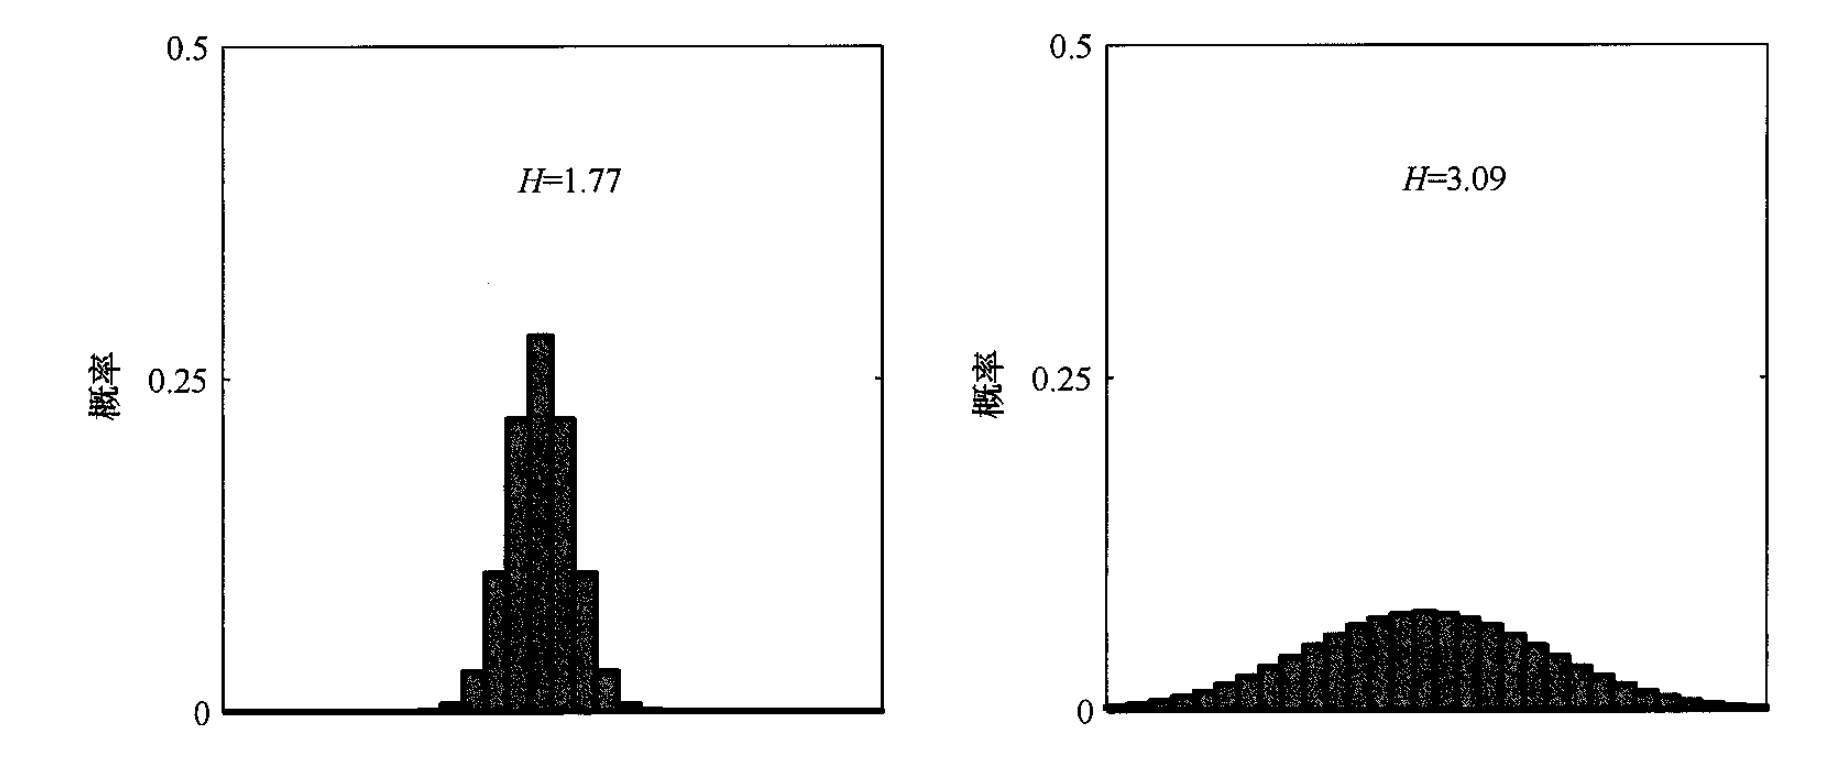
\includegraphics[width=0.9\textwidth]{ch02-fig2-14-entropy-hist.png}
  \caption{$30$ 个分箱上两种概率分布的直方图说明了更宽的分布具有更大的熵 $H$。最大的熵来自均匀分布，它使 $H=-\ln\frac{1}{30}=3.40$。}
  \label{figure:ch02-两种熵}
\end{figure}

我们可以发现所有的 $p(x_i)$ 都是相等的，且由 $p(x_i)=1/M$ 给出，其中 $M$ 是状态 $x_i$ 的总数。然后熵的相应值是 $H=\ln M$（见\cref{exercise:ch02-22}）。这个结果也可以从 Jensen 不等式（下文将很快讨论它）得出（见\cref{exercise:ch02-23}）。为了验证驻点确实是一个最大值，可以计算熵的二阶导数，得到

\begin{align}
  \frac{\partial^{2}\tilde{H}}{\partial p(x_i)\,\partial p(x_j)} = -I_{ij}\frac{1}{p_i}
  \label{align:ch02-熵二阶导}
\end{align}

其中，$I_{ij}$ 是单位矩阵的元素。可以看到这些值都是负的，因此驻点确实是一个极大值。

\begin{proposition}[均匀分布使熵最大]\label{proposition:ch02-均匀最大熵}
设离散随机变量 $x$ 有 $M$ 个可能取值，则 $\sum_ip_i=1$、$p_i\geqslant0$ 的约束下，\eqref{align:ch02-离散熵}（以自然对数计）在 $p_i=1/M$（对一切 $i$）处取最大值，最大值为 $H=\ln M$。
\end{proposition}

\begin{proof}
考虑 Lagrange 函数\eqref{align:ch02-熵Lagrange}。对 $p(x_i)$ 求偏导并令其为零：
\begin{align*}
  \frac{\partial\tilde{H}}{\partial p(x_i)} = -\ln p(x_i) - 1 + \lambda = 0
  \quad\Longrightarrow\quad
  p(x_i) = e^{\lambda-1} ,
\end{align*}
即所有 $p(x_i)$ 相等。再由约束 $\sum_ip_i=1$ 得 $Me^{\lambda-1}=1$，故 $p(x_i)=1/M$。此时
\begin{align*}
  H = -\sum_{i=1}^{M}\frac{1}{M}\ln\frac{1}{M} = \ln M .
\end{align*}
最后验证它是极大值：由\eqref{align:ch02-熵二阶导}，Hessian 为对角矩阵，对角元 $-1/p_i<0$，故为负定，驻点即最大值点。
\end{proof}

% SUPPLEMENT: parent=proposition:ch02-均匀最大熵; kind=motivation; location=紧随其后的 remark（重构新增）
\begin{remark}（重构新增）
这条结果给出了“熵最大”的精确含义：在只知道取值个数、不知道其他任何信息时，最不偏不倚的选择就是均匀分布。这与\cref{figure:ch02-两种熵}中右侧那个更平的直方图对应，也是“最大熵原理”在离散情形下的全部内容。

条件的清单要看清：约束只有两条——归一化 $\sum p_i=1$ 与非负性 $p_i\geqslant0$。若再加约束（例如规定均值），最大值就会变成指数族分布而不是均匀分布（见\cref{subsection:ch02-最大熵}的连续版本）。二阶导验证不可省：一阶条件只给出驻点，\eqref{align:ch02-熵二阶导}才把它确认为最大值。
\end{remark}

\subsection{微分熵}\label{subsection:ch02-微分熵}

我们可以将熵的定义扩展到连续变量 $x$ 的分布 $p(x)$ 上。首先将 $x$ 分成宽度为 $\Delta$ 的区间，然后假设 $p(x)$ 是连续的，中值定理（mean value theorem）（Weinstein, 1999）告诉我们，对于每个这样的区间，必定存在一个值 $x_i$ 在范围 $i\Delta\leqslant x_i\leqslant(i+1)\Delta$ 内，使得

\begin{align}
  \int_{i\Delta}^{(i+1)\Delta} p(x)\,\mathrm{d}x = p(x_i)\Delta
  \label{align:ch02-中值定理}
\end{align}

现在我们可以通过将任何落入第 $i$ 个区间的值 $x$ 赋予 $x_i$ 来量化连续变量 $x$。观察到值 $x_i$ 的概率是 $p(x_i)\Delta$。这给出了一个离散分布，其熵的形式为

\begin{align}
  H_{\Delta} = -\sum_i p(x_i)\Delta\ln\big(p(x_i)\Delta\big) = -\sum_i p(x_i)\Delta\ln p(x_i) - \ln\Delta
  \label{align:ch02-离散化熵}
\end{align}

其中 $\sum_ip(x_i)\Delta=1$，这是由\eqref{align:ch02-中值定理}和\eqref{align:ch02-密度归一化}得出的。现在忽略\eqref{align:ch02-离散化熵}右侧的第二项 $-\ln\Delta$，因为它与 $p(x)$ 无关，然后考虑极限 $\Delta\to0$。在此极限下，\eqref{align:ch02-离散化熵}右侧的第一项将趋近于 $p(x)\ln p(x)$ 的积分，因此有

\begin{align}
  \lim_{\Delta\to0}\left\{-\sum_i p(x_i)\Delta\ln p(x_i)\right\} = -\int p(x)\ln p(x)\,\mathrm{d}x
  \label{align:ch02-微分熵极限}
\end{align}

\begin{definition}[微分熵]\label{definition:ch02-微分熵}
称\eqref{align:ch02-微分熵极限}右端的量 $-\int p(x)\ln p(x)\,\mathrm{d}x$ 为连续随机变量 $x$ 的\textbf{微分熵}（differential entropy）。对于定义在多个连续变量上的密度（统一用向量 $\mathbf{x}$ 表示），微分熵为
\begin{align*}
  H[\mathbf{x}] = -\int p(\mathbf{x})\ln p(\mathbf{x})\,\mathrm{d}\mathbf{x} .
\end{align*}
\end{definition}

% SUPPLEMENT: parent=definition:ch02-微分熵; kind=motivation; location=紧随其后的 remark（重构新增）
\begin{remark}（重构新增）
微分熵是把熵的定义“先离散化、再取极限”得到的：\eqref{align:ch02-离散化熵}右侧的第一项在 $\Delta\to0$ 时收敛，第二项 $-\ln\Delta$ 却发散，因此微分熵只保留了收敛的那部分。代价是它不再具有离散熵的直观含义（不是“比特数”），并且可以为负。

这一点在\eqref{align:ch02-Gauss熵}中会看到：当 $\sigma^{2}<1/(2\pi e)$ 时微分熵为负。尽管有这一缺陷，微分熵在比较同一坐标系下的不同分布时仍然有用，也是 KL 散度与最大熵推导的基础。
\end{remark}

式\eqref{align:ch02-微分熵极限}右侧的量称为微分熵（differential entropy）。我们可以看到，离散形式和连续形式的熵的不同之处在于 $\ln\Delta$，而它在极限 $\Delta\to0$ 下是发散的。这表明非常精确地描述一个连续变量需要大量比特位。

\subsection{最大熵}\label{subsection:ch02-最大熵}

我们已经看到，对于离散分布，最大熵的情况对应变量概率在可能状态之间均匀分布的情况。现在我们来考虑连续变量的对应结果。如果要明确定义这个最大值，则需要约束 $p(x)$ 的一阶矩和二阶矩，并保持归一化约束。因此，我们需要在以下 $3$ 个约束下最大化微分熵：

\begin{align}
  \int_{-\infty}^{\infty} p(x)\,\mathrm{d}x = 1
  \label{align:ch02-最大熵约束1}
\end{align}

\begin{align}
  \int_{-\infty}^{\infty} x\,p(x)\,\mathrm{d}x = \mu
  \label{align:ch02-最大熵约束2}
\end{align}

\begin{align}
  \int_{-\infty}^{\infty} (x-\mu)^{2}p(x)\,\mathrm{d}x = \sigma^{2}
  \label{align:ch02-最大熵约束3}
\end{align}

可以使用 Lagrange 乘子法来进行带约束的最大化（参见\cref{chapter:appC-Lagrange乘子}），为此需要最大化以下关于 $p(x)$ 的函数：

\begin{align}
  & -\int_{-\infty}^{\infty} p(x)\ln p(x)\,\mathrm{d}x + \lambda_1\left(\int_{-\infty}^{\infty} p(x)\,\mathrm{d}x - 1\right) \nonumber \\
  & \quad + \lambda_2\left(\int_{-\infty}^{\infty} x\,p(x)\,\mathrm{d}x - \mu\right) + \lambda_3\left(\int_{-\infty}^{\infty}(x-\mu)^{2}p(x)\,\mathrm{d}x - \sigma^{2}\right)
  \label{align:ch02-最大熵泛函}
\end{align}

使用变分法（参见\cref{chapter:appB-变分法}），令上述函数的导数为零，可以得到

\begin{align}
  p(x) = \exp\left\{-1 + \lambda_1 + \lambda_2 x + \lambda_3(x-\mu)^{2}\right\}
  \label{align:ch02-最大熵形式}
\end{align}

通过将这个结果代回 $3$ 个约束方程可以得到 Lagrange 乘子，最终得到如下结果（见\cref{exercise:ch02-24}）：

\begin{align}
  p(x) = \frac{1}{\sqrt{2\pi\sigma^{2}}}\exp\left(-\frac{(x-\mu)^{2}}{2\sigma^{2}}\right)
  \label{align:ch02-最大熵Gauss}
\end{align}

\begin{theorem}[最大熵分布是 Gauss 分布]\label{theorem:ch02-最大熵Gauss}
在约束\eqref{align:ch02-最大熵约束1}、\eqref{align:ch02-最大熵约束2}、\eqref{align:ch02-最大熵约束3}下，使微分熵最大的密度由\eqref{align:ch02-最大熵Gauss}给出，即均值为 $\mu$、方差为 $\sigma^{2}$ 的 Gauss 分布。
\end{theorem}

\begin{proof}
对\eqref{align:ch02-最大熵泛函}关于 $p(x)$ 作变分，令其为零：
\begin{align*}
  \frac{\delta}{\delta p(x)}\Big[-\int p\ln p\,\mathrm{d}x + \lambda_1\!\int p\,\mathrm{d}x + \lambda_2\!\int xp\,\mathrm{d}x + \lambda_3\!\int(x-\mu)^{2}p\,\mathrm{d}x\Big]
  = -\ln p(x) - 1 + \lambda_1 + \lambda_2x + \lambda_3(x-\mu)^{2} = 0 ,
\end{align*}
即得\eqref{align:ch02-最大熵形式}。把\eqref{align:ch02-最大熵形式}代入三个约束：由\eqref{align:ch02-最大熵约束3}，$\lambda_3$ 必须为负（否则\eqref{align:ch02-最大熵约束1}的积分发散），记 $\lambda_3=-1/(2\sigma^{2})$，则\eqref{align:ch02-最大熵形式}成为 Gauss 分布的二次指数形式；再由\eqref{align:ch02-最大熵约束2}，线性项的中心为 $\mu$（即 $\lambda_2=\mu/\sigma^{2}$ 时均值为 $\mu$）；最后由\eqref{align:ch02-最大熵约束1}定出归一化常数，得\eqref{align:ch02-最大熵Gauss}。约束\eqref{align:ch02-最大熵约束3}同时给出二次项的系数，故方差确为 $\sigma^{2}$。
\end{proof}

% SUPPLEMENT: parent=theorem:ch02-最大熵Gauss; kind=motivation; location=紧随其后的 remark（重构新增）
\begin{remark}（重构新增）
这条定理解释了\cref{section:ch02-Gauss分布}开头那句话：Gauss 分布不是“形式任意”的，而是在只固定前两阶矩时最不偏不倚的选择。这也是为什么在许多模型中默认采用 Gauss 噪声——它在线索最少时引入了最少的额外假设。

三个约束缺一不可：若去掉\eqref{align:ch02-最大熵约束3}，最大熵解不存在（可把方差推向无穷使熵任意增大）；若去掉\eqref{align:ch02-最大熵约束2}，解仍为 Gauss 但中心不确定；若去掉\eqref{align:ch02-最大熵约束1}，则连归一化都无法保证。定理的证明只用到变分法，但结果确实满足 $p(x)\geqslant0$，因此在最大化时无需额外施加非负约束。
\end{remark}

因此，最大化微分熵的分布是 Gauss 分布。注意，在最大化熵时我们没有限制分布是非负的。然而，结果分布确实是非负的，事后看来这样的约束是不必要的。

如果我们计算 Gauss 分布的微分熵，则可以得到（见\cref{exercise:ch02-25}）

\begin{align}
  H[x] = \frac{1}{2}\left(1+\ln(2\pi\sigma^{2})\right)
  \label{align:ch02-Gauss熵}
\end{align}

\begin{proposition}[Gauss 分布的微分熵]\label{proposition:ch02-Gauss熵}
设 $x\sim\mathcal{N}(x\mid\mu,\sigma^{2})$，则其微分熵由\eqref{align:ch02-Gauss熵}给出。
\end{proposition}

\begin{proof}
把\eqref{align:ch02-单变量Gauss}代入微分熵的定义并利用 $\int p=1$：
\begin{align*}
  H[x] &= -\int p(x)\left[-\frac{1}{2}\ln(2\pi\sigma^{2}) - \frac{(x-\mu)^{2}}{2\sigma^{2}}\right]\mathrm{d}x \\
  &= \frac{1}{2}\ln(2\pi\sigma^{2})\int p(x)\,\mathrm{d}x + \frac{1}{2\sigma^{2}}\int(x-\mu)^{2}p(x)\,\mathrm{d}x \\
  &= \frac{1}{2}\ln(2\pi\sigma^{2}) + \frac{1}{2\sigma^{2}}\cdot\sigma^{2} = \frac{1}{2}\left(1+\ln(2\pi\sigma^{2})\right),
\end{align*}
其中第三个等号用了\eqref{align:ch02-最大熵约束3}。
\end{proof}

% SUPPLEMENT: parent=proposition:ch02-Gauss熵; kind=motivation; location=紧随其后的 remark（重构新增）
\begin{remark}（重构新增）
这条结果把“熵”与“方差”直接联系起来：方差越大，熵越大，这与\cref{figure:ch02-两种熵}的直观一致。它也给出微分熵可以为负的明确阈值：当 $\sigma^{2}<1/(2\pi e)$ 时 $H[x]<0$，而与离散熵的非负性形成对照。

推导依赖\eqref{align:ch02-最大熵约束3}（即二阶中心矩等于 $\sigma^{2}$），这一步同时用到了\cref{proposition:ch02-Gauss矩}的结论。注意公式只依赖 $\sigma^{2}$ 而不依赖 $\mu$：平移不改变熵，这与离散熵对标签重命名不变是同一回事。
\end{remark}

我们可以再次看到，随着分布变得更宽（即 $\sigma^{2}$ 增加），熵也增加。这个结果还表明，与离散熵不同，微分熵可以是负的，因为当 $\sigma^{2}<1/(2\pi e)$ 时，\eqref{align:ch02-Gauss熵}中的 $H(x)<0$。

\subsection{Kullback-Leibler 散度}\label{subsection:ch02-KL散度}

到目前为止，我们已经介绍了信息论中的许多概念，包括熵的关键符号表示。下面让我们将这些想法与机器学习联系起来。考虑某个未知分布 $p(x)$，并假设我们使用了一个近似分布 $q(x)$ 来对它进行建模。如果使用 $q(x)$ 来构建编码方案以便向接收者传输 $x$ 的值，那么由于使用 $q(x)$ 而不是真实分布 $p(x)$（假设我们选择了一种高效的编码方案），描述 $x$ 值所需的平均额外（additional）信息量（单位：纳特）可由下式给出：

\begin{align}
  \mathrm{KL}(p\|q) = -\int p(x)\ln q(x)\,\mathrm{d}x - \left(-\int p(x)\ln p(x)\,\mathrm{d}x\right) = -\int p(x)\ln\frac{q(x)}{p(x)}\,\mathrm{d}x
  \label{align:ch02-kl散度}
\end{align}

\begin{definition}[Kullback-Leibler 散度]\label{definition:ch02-kl散度}
称由\eqref{align:ch02-kl散度}定义的量为分布 $p(x)$ 与 $q(x)$ 之间的\textbf{相对熵}（relative entropy），又称 \textbf{Kullback-Leibler} 散度（Kullback-Leibler divergence），简称 \textbf{KL} 散度（Kullback and Leibler, 1951）。它度量用 $q$ 代替 $p$ 时所需的平均额外信息量。
\end{definition}

% SUPPLEMENT: parent=definition:ch02-kl散度; kind=motivation; location=紧随其后的 remark（重构新增）
\begin{remark}（重构新增）
KL 散度的定义来自“编码代价之差”：用真实分布 $p$ 编码的期望码长是 $-\int p\ln p$（即微分熵），用近似分布 $q$ 编码的期望码长是 $-\int p\ln q$，两者之差就是\eqref{align:ch02-kl散度}。因此它不是对称的：$q$ 在 $p$ 的支撑集上取小值会受到重罚，反之则不会。

这种不对称性是 KL 散度的固有性质（$\mathrm{KL}(p\|q)\neq\mathrm{KL}(q\|p)$），使用时必须明确“谁是真值、谁是近似”。此外，\eqref{align:ch02-kl散度}要求 $p,q$ 都归一化，否则右端会多出与归一化常数有关的项；在变分推断中常见的 ELBO 就是在这种非归一化情形下使用的。
\end{remark}

这就是分布 $p(x)$ 和 $q(x)$ 之间的相对熵（relative entropy），又称 Kullback-Leibler 散度（Kullback-Leibler divergence），简称 KL 散度（Kullback and Leibler, 1951）。注意，它不是一个对称量，也就是说，$\mathrm{KL}(p\|q)\neq\mathrm{KL}(q\|p)$。

Kullback-Leibler 散度满足 $\mathrm{KL}(p\|q)\geqslant0$，当且仅当 $p(x)=q(x)$ 时等式成立。为了进行证明，我们首先引入凸（convex）函数的概念。如\cref{figure:ch02-凸函数}所示，如果函数 $f(x)$ 具有每条弦都位于函数上方或与函数重合的性质，则称该函数是凸的。

\begin{definition}[凸函数与凹函数]\label{definition:ch02-凸函数}
若函数 $f$ 满足：对任意 $a,b$ 与任意 $0\leqslant\lambda\leqslant1$，
\begin{align*}
  f\big(\lambda a+(1-\lambda)b\big) \leqslant \lambda f(a)+(1-\lambda)f(b) ,
\end{align*}
即每条弦都位于函数图像上方或与图像重合，则称 $f$ 是\textbf{凸的}（convex）。若上式对 $\lambda\in(0,1)$ 严格成立（除 $a=b$ 外），则称 $f$ 是\textbf{严格凸的}（strictly convex）。若 $-f$ 是凸的，则称 $f$ 是\textbf{凹的}（concave），相应地有严格凹函数。
\end{definition}

% SUPPLEMENT: parent=definition:ch02-凸函数; kind=motivation; location=紧随其后的 remark（重构新增）
\begin{remark}（重构新增）
凸性刻画的是“函数图像向下弯”：弦在图像上方意味着函数值的增长越来越快（二阶导非负）。这一性质的价值在于它保证局部极小就是全局极小，从而使优化问题变简单；在信息论中，它则是证明 KL 散度非负的关键。

定义中的 $\lambda$ 可以解释为 $a,b$ 之间的插值权重：$\lambda a+(1-\lambda)b$ 遍历区间 $[a,b]$。注意凸性要求对\textbf{所有} $\lambda$ 成立，只在个别点成立不叫凸。若 $f$ 二阶可导，凸性等价于 $f''\geqslant0$（见\cref{exercise:ch02-32}），这也是实际检验时最常用的判据。
\end{remark}

任何处在 $x=a$ 到 $x=b$ 区间中的 $x$ 值都可以写成 $\lambda a+(1-\lambda)b$ 的形式，其中 $0\leqslant\lambda\leqslant1$。弦上对应的点由 $\lambda f(a)+(1-\lambda)f(b)$ 给出，函数的对应值是 $f(\lambda a+(1-\lambda)b)$。函数 $f(x)$ 是凸的意味着

\begin{align}
  f\big(\lambda a+(1-\lambda)b\big) \leqslant \lambda f(a)+(1-\lambda)f(b)
  \label{align:ch02-凸函数定义}
\end{align}

这等价于要求函数的二阶导数在任何地方都是正的（见\cref{exercise:ch02-32}）。凸函数的例子有 $x\ln x$（$x>0$）和 $x^{2}$。如果一个函数仅在 $\lambda=0$ 和 $\lambda=1$ 时 KL$(p\|q)=0$ 成立，则称其为严格凸的（strictly convex）。如果一个函数具有相反的性质，即每条弦都位于函数之下或与函数重合，则称其为凹的（concave），对应也存在严格凹的（strictly concave）函数。如果函数 $f(x)$ 是凸的，那么 $-f(x)$ 是凹的。

\begin{remark}（重构新增）原文问题说明
上一段中“如果一个函数仅在 $\lambda=0$ 和 $\lambda=1$ 时 KL$(p\|q)=0$ 成立，则称其为严格凸的”一句，原书把“等号”误印成了 KL$(p\|q)=0$：严格凸的定义与 KL 散度无关，正确表述应为“若\eqref{align:ch02-凸函数定义}中的等号仅在 $\lambda=0$ 和 $\lambda=1$ 时成立，则称 $f$ 为严格凸的”。正文照录原文，特此说明；后文凡涉及严格凸性的论证均按上述正确表述使用。
\end{remark}

\begin{figure}[htbp]
  \centering
  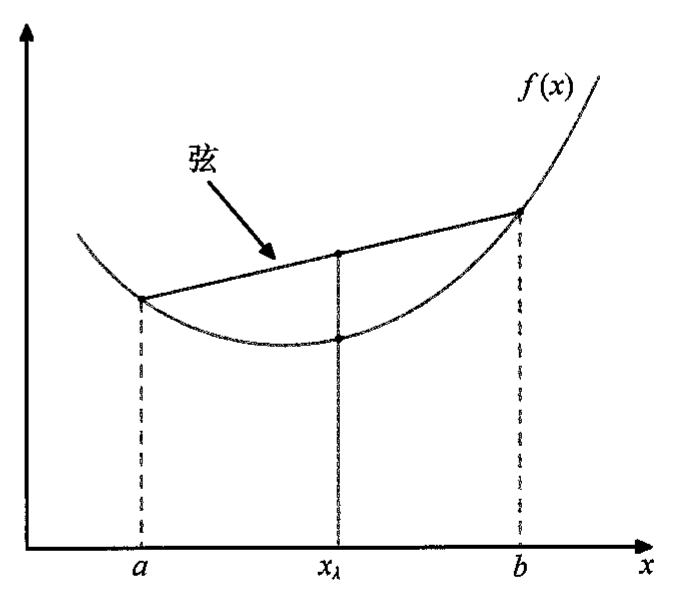
\includegraphics[width=0.5\textwidth]{ch02-fig2-15-convex.png}
  \caption{凸函数 $f(x)$ 的每条弦（蓝色）都位于函数（红色）之上或与函数重合。}
  \label{figure:ch02-凸函数}
\end{figure}

使用归纳法，从\eqref{align:ch02-凸函数定义}可以得到（见\cref{exercise:ch02-33}）如下结论：对于任何一组点 $\{x_i\}$，凸函数 $f(x)$ 须满足

\begin{align}
  f\left(\sum_{i=1}^{M}\lambda_i x_i\right) \leqslant \sum_{i=1}^{M}\lambda_i f(x_i)
  \label{align:ch02-jensen离散}
\end{align}

其中 $\lambda_i\geqslant0$ 且 $\sum_{i=1}^{M}\lambda_i=1$。\eqref{align:ch02-jensen离散}称为 Jensen 不等式（Jensen's inequality）。如果我们将 $\lambda_i$ 解释为离散变量 $x$ 在 $\{x_i\}$ 上取值的概率分布，则\eqref{align:ch02-jensen离散}可以写成

\begin{align}
  f\big(\mathbb{E}[x]\big) \leqslant \mathbb{E}\big[f(x)\big]
  \label{align:ch02-jensen期望}
\end{align}

其中 $\mathbb{E}[\cdot]$ 表示期望。对于连续变量，Jensen 不等式具有以下形式：

\begin{align}
  f\left(\int x\,p(x)\,\mathrm{d}x\right) \leqslant \int f(x)\,p(x)\,\mathrm{d}x
  \label{align:ch02-jensen连续}
\end{align}

\begin{theorem}[Jensen 不等式]\label{theorem:ch02-jensen}
设 $f$ 为凸函数，$\lambda_i\geqslant0$、$\sum_i\lambda_i=1$，则\eqref{align:ch02-jensen离散}成立；若 $x$ 为随机变量，则\eqref{align:ch02-jensen期望}与\eqref{align:ch02-jensen连续}成立，即 $f(\mathbb{E}[x])\leqslant\mathbb{E}[f(x)]$。
\end{theorem}

\begin{proof}
先对 $M$ 作归纳证明\eqref{align:ch02-jensen离散}。$M=1$ 时两边相等；$M=2$ 时即\eqref{align:ch02-凸函数定义}。设结论对 $M-1$ 成立，则对 $M$ 项（不妨设 $\lambda_M<1$），令 $\Lambda=\sum_{i=1}^{M-1}\lambda_i=1-\lambda_M$，
\begin{align*}
  f\left(\sum_{i=1}^{M}\lambda_ix_i\right)
  &= f\left(\Lambda\cdot\sum_{i=1}^{M-1}\frac{\lambda_i}{\Lambda}x_i + \lambda_Mx_M\right)
  \leqslant \Lambda\,f\left(\sum_{i=1}^{M-1}\frac{\lambda_i}{\Lambda}x_i\right) + \lambda_Mf(x_M) \\
  &\leqslant \Lambda\sum_{i=1}^{M-1}\frac{\lambda_i}{\Lambda}f(x_i) + \lambda_Mf(x_M)
  = \sum_{i=1}^{M}\lambda_if(x_i) ,
\end{align*}
其中第一个不等号用了 $M=2$ 的凸性，第二个用了归纳假设（注意 $\lambda_i/\Lambda$ 仍非负且和为 $1$）。

\eqref{align:ch02-jensen期望}是\eqref{align:ch02-jensen离散}在 $\lambda_i=p(x_i)$、$M\to\infty$ 时的写法；\eqref{align:ch02-jensen连续}则把求和换成积分，证明方式相同（把积分看作和的极限）。
\end{proof}

% SUPPLEMENT: parent=theorem:ch02-jensen; kind=motivation; location=紧随其后的 remark（重构新增）
\begin{remark}（重构新增）
Jensen 不等式是信息论中几乎所有非负性结论的统一来源：KL 散度非负、互信息非负、最大熵的解是 Gauss 分布，都可由它推出。直观上，它说的是“先平均再取凸函数”不大于“先取凸函数再平均”。

条件“$f$ 凸”不可省：对凹函数不等号反向（$f(\mathbb{E}[x])\geqslant\mathbb{E}[f(x)]$）。条件“$\lambda_i\geqslant0$、$\sum\lambda_i=1$”也不可省，它保证 $\sum\lambda_ix_i$ 是凸组合，从而落在 $f$ 的定义域内。若 $f$ 严格凸，等号仅在 $x$ 几乎必然为常数时成立。
\end{remark}

我们可以将\eqref{align:ch02-jensen连续}所示形式的 Jensen 不等式应用于 Kullback-Leibler 散度［见\eqref{align:ch02-kl散度}］，得到

\begin{align}
  \mathrm{KL}(p\|q) = -\int p(x)\ln\frac{q(x)}{p(x)}\,\mathrm{d}x \geqslant -\ln\int q(x)\,\mathrm{d}x = 0
  \label{align:ch02-kl非负}
\end{align}

\begin{proposition}[KL 散度的非负性]\label{proposition:ch02-kl非负}
设 $p,q$ 为概率密度，则 $\mathrm{KL}(p\|q)\geqslant0$，且等号成立当且仅当 $p(x)=q(x)$（几乎处处）。
\end{proposition}

\begin{proof}
在\eqref{align:ch02-jensen连续}中取 $f(u)=-\ln u$（它是凸函数，见\cref{exercise:ch02-32}），并取随机变量 $u=q(x)/p(x)$、其分布由 $p$ 给出，则
\begin{align*}
  \mathrm{KL}(p\|q) = -\int p(x)\ln\frac{q(x)}{p(x)}\,\mathrm{d}x
  = \mathbb{E}_p\big[-\ln u\big]
  \geqslant -\ln\mathbb{E}_p[u]
  = -\ln\int p(x)\frac{q(x)}{p(x)}\,\mathrm{d}x = -\ln\int q(x)\,\mathrm{d}x = 0 .
\end{align*}
若 $p=q$，被积函数 $\ln(q/p)=\ln1=0$，故 $\mathrm{KL}=0$。反之，若 $\mathrm{KL}=0$，则 Jensen 不等式取等号；由 $-\ln$ 严格凸，这要求 $u=q(x)/p(x)$ 在 $p(x)>0$ 处为常数，结合双方归一化得该常数为 $1$，即 $p=q$（几乎处处）。
\end{proof}

% SUPPLEMENT: parent=proposition:ch02-kl非负; kind=motivation; location=紧随其后的 remark（重构新增）
\begin{remark}（重构新增）
非负性是 KL 散度被称为“散度”的资格：它度量两个分布的不相似程度，且最小值 $0$ 只在两个分布相同时取到。证明只用了一步——把 $-\ln$ 的凸性代入 Jensen 不等式——却给出了整个信息论中最常用的不等式。

条件“$p,q$ 都归一化”在证明的最后一个等号中用到（$\int q=1$）；若 $q$ 未归一化，则 $\mathrm{KL}(p\|q)\geqslant-\ln\int q$，可以为负。此外，若 $q(x)=0$ 而 $p(x)>0$ 在某个正测度集上成立，则 $\mathrm{KL}=+\infty$，此时不等式仍成立（广义实数意义下）。
\end{remark}

其中利用了 $-\ln x$ 是凸函数这一性质，并且利用了归一化条件 $\int q(x)\,\mathrm{d}x=1$。实际上，$-\ln x$ 是严格凸函数，所以当且仅当对所有 $x$ 有 $q(x)=p(x)$ 时等式成立。可以将 Kullback-Leibler 散度解释为对两个分布 $p(x)$ 和 $q(x)$ 不相似度的度量。

可以看到，数据压缩和密度估计（建模未知概率分布的问题）之间有着密切的关系，因为当我们知道真实分布时，就可以实现最有效的压缩。如果我们使用与真实分布不同的分布，那么最终只能得到一种效率较低的编码方式，并且平均来说，必须传输的额外信息（至少）等于两个分布之间的 Kullback-Leibler 散度。

假设数据是从一个我们希望建模的未知分布 $p(x)$ 中产生的。我们可以尝试使用由一组可调参数 $\boldsymbol{\theta}$ 控制的参数化分布 $q(x\mid\boldsymbol{\theta})$ 来近似这个分布。确定 $\boldsymbol{\theta}$ 的一种方法是最小化 $p(x)$ 和 $q(x\mid\boldsymbol{\theta})$ 之间的 Kullback-Leibler 散度。但是由于我们不知道 $p(x)$，因此无法直接做到这一点。然而，假设我们已经观察到一组有限的训练点——从 $p(x)$ 中产生的 $x_n$，其中 $n=1,\cdots,N$，则可以使用\eqref{align:ch02-样本近似}，通过这些训练点上的有限和来近似关于 $p(x)$ 的期望：

\begin{align}
  \mathrm{KL}(p\|q) \approx \frac{1}{N}\sum_{n=1}^{N}\big(-\ln q(x_n\mid\boldsymbol{\theta}) + \ln p(x_n)\big)
  \label{align:ch02-kl样本近似}
\end{align}

式\eqref{align:ch02-kl样本近似}右侧的第二项与 $\boldsymbol{\theta}$ 无关，第一项是分布 $q(x\mid\boldsymbol{\theta})$ 使用训练集评估时 $\boldsymbol{\theta}$ 的负对数似然函数。因此可以看到，最小化这个 Kullback-Leibler 散度等同于最大化对数似然函数（见\cref{exercise:ch02-34}）。

\begin{proposition}[KL 散度与对数似然]\label{proposition:ch02-kl与似然}
设 $q(x\mid\boldsymbol{\theta})$ 为参数化密度，则关于 $\boldsymbol{\theta}$ 最小化 $\mathrm{KL}(p\|q)$ 等价于关于 $\boldsymbol{\theta}$ 最大化期望对数似然 $\mathbb{E}_p[\ln q(x\mid\boldsymbol{\theta})]$；在样本近似\eqref{align:ch02-kl样本近似}下等价于最大化 $\sum_n\ln q(x_n\mid\boldsymbol{\theta})$。
\end{proposition}

\begin{proof}
把\eqref{align:ch02-kl散度}拆开：
\begin{align*}
  \mathrm{KL}(p\|q) = -\int p(x)\ln q(x\mid\boldsymbol{\theta})\,\mathrm{d}x + \int p(x)\ln p(x)\,\mathrm{d}x .
\end{align*}
右端第二项与 $\boldsymbol{\theta}$ 无关，故最小化左端等价于最大化第一项，即 $\mathbb{E}_p[\ln q(x\mid\boldsymbol{\theta})]$。再用\eqref{align:ch02-样本近似}把该期望换成样本平均 $\frac{1}{N}\sum_n\ln q(x_n\mid\boldsymbol{\theta})$，乘以常数 $N$ 不影响最优点，即得第二种表述。
\end{proof}

% SUPPLEMENT: parent=proposition:ch02-kl与似然; kind=motivation; location=紧随其后的 remark（重构新增）
\begin{remark}（重构新增）
这条等价性是“最大似然 = 最小 KL”的精确版本，它把\cref{subsection:ch02-似然函数}中的似然方法与信息论联系起来：选择模型时，我们实际上是在让模型分布尽量靠近真实分布。

条件“$p$ 固定”不可省：$p$ 决定了 KL 散度中不可优化的那一项，因此最小化只对 $\boldsymbol{\theta}$ 进行。若用有限样本近似\eqref{align:ch02-样本近似}，则所得解是最大似然解，它的抽样误差由 $N$ 控制——这也解释了为什么数据越多，学到的分布越接近真值。
\end{remark}

\subsection{条件熵}\label{subsection:ch02-条件熵}

现在考虑两组变量 $x$ 和 $y$ 之间的联合分布 $p(x,y)$，从中采样 $x$ 和 $y$ 的值对。如果 $x$ 的值已知，那么明确对应 $y$ 值所需的额外信息由 $-\ln p(y\mid x)$ 给出。因此，明确 $y$ 所需的平均额外信息可以写成

\begin{align}
  H[y\mid x] = -\iint p(y,x)\ln p(y\mid x)\,\mathrm{d}y\,\mathrm{d}x
  \label{align:ch02-条件熵}
\end{align}

\begin{definition}[条件熵]\label{definition:ch02-条件熵}
称由\eqref{align:ch02-条件熵}定义的量 $H[y\mid x]$ 为给定 $x$ 的条件下 $y$ 的\textbf{条件熵}（conditional entropy），它表示在已知 $x$ 后描述 $y$ 平均所需的额外信息量。
\end{definition}

% SUPPLEMENT: parent=definition:ch02-条件熵; kind=motivation; location=紧随其后的 remark（重构新增）
\begin{remark}（重构新增）
条件熵是“在已知 $x$ 之后还剩多少不确定性”，因此它必然不大于无条件熵（\cref{exercise:ch02-29}）。这个差别正是互信息（\cref{subsection:ch02-互信息}）要量化的东西。

\eqref{align:ch02-条件熵}中的 $-\ln p(y\mid x)$ 用的是条件密度而不是联合密度，这是它与联合熵的唯一差别；求和（积分）仍然按联合分布 $p(x,y)$ 加权，因为实际观测到的 $(x,y)$ 就是按联合分布出现的。条件 $p(x)>0$ 不可省，否则 $p(y\mid x)$ 无定义。
\end{remark}

$H[y\mid x]$ 称为给定 $x$ 的条件下 $y$ 的条件熵（conditional entropy）。应用乘积法则容易看出，条件熵满足如下关系（见\cref{exercise:ch02-35}）：

\begin{align}
  H[x,y] = H[y\mid x] + H[x]
  \label{align:ch02-熵链式}
\end{align}

其中 $H[x,y]$ 是 $p(x,y)$ 的微分熵，$H[x]$ 是边缘分布 $p(x)$ 的微分熵。因此，描述 $x$ 和 $y$ 所需的信息实际就是描述 $x$ 本身所需的信息再加上给定 $x$ 描述 $y$ 所需的额外信息。

\begin{proposition}[熵的链式法则]\label{proposition:ch02-熵链式}
设 $p(x,y)$ 为联合密度，$p(x)$、$p(y\mid x)$ 为相应的边缘与条件密度，则\eqref{align:ch02-熵链式}成立。
\end{proposition}

\begin{proof}
由 $p(x,y)=p(y\mid x)p(x)$（\eqref{align:ch02-连续乘积法则}）取对数得 $\ln p(x,y)=\ln p(y\mid x)+\ln p(x)$。两边乘以 $-p(x,y)$ 并对 $(x,y)$ 积分：
\begin{align*}
  H[x,y] &= -\iint p(x,y)\ln p(x,y)\,\mathrm{d}x\,\mathrm{d}y \\
  &= -\iint p(x,y)\ln p(y\mid x)\,\mathrm{d}x\,\mathrm{d}y - \iint p(x,y)\ln p(x)\,\mathrm{d}x\,\mathrm{d}y .
\end{align*}
第一项即 $H[y\mid x]$。第二项中 $\ln p(x)$ 与 $y$ 无关，对 $y$ 积分得 $\int p(x)\ln p(x)\,\mathrm{d}x$ 的相反数，即 $H[x]$。故\eqref{align:ch02-熵链式}成立。
\end{proof}

% SUPPLEMENT: parent=proposition:ch02-熵链式; kind=motivation; location=紧随其后的 remark（重构新增）
\begin{remark}（重构新增）
链式法则把“联合的不确定性”分解为“$x$ 的不确定性”加“已知 $x$ 后 $y$ 剩余的不确定性”，这与乘积法则把联合概率分解为两步完全平行——事实上证明就是乘积法则取对数。

它的直接推论是 $H[x,y]\leqslant H[x]+H[y]$（\cref{exercise:ch02-29}），等号当且仅当 $x,y$ 独立。条件“$p(x)>0$”用于保证 $p(y\mid x)$ 有定义；若某个 $x$ 取值的概率为零，该处对积分的贡献也为零，不影响结论。
\end{remark}

\subsection{互信息}\label{subsection:ch02-互信息}

当两个变量 $x$ 和 $y$ 独立时，它们的联合分布便可以分解为它们边缘分布的乘积，即 $p(x,y)=p(x)p(y)$。如果这两个变量不独立，则可以通过考虑联合分布和边缘分布乘积之间的 Kullback-Leibler 散度来了解它们是否“接近”独立，其由下式给出：

\begin{align}
  I[x,y] = \mathrm{KL}\big(p(x,y)\,\|\,p(x)p(y)\big) = -\iint p(x,y)\ln\frac{p(x)p(y)}{p(x,y)}\,\mathrm{d}x\,\mathrm{d}y
  \label{align:ch02-互信息}
\end{align}

\begin{definition}[互信息]\label{definition:ch02-互信息}
称由\eqref{align:ch02-互信息}定义的量 $I[x,y]$ 为变量 $x$ 与 $y$ 之间的\textbf{互信息}（mutual information），它是联合分布 $p(x,y)$ 与其边缘分布之积 $p(x)p(y)$ 之间的 KL 散度。
\end{definition}

% SUPPLEMENT: parent=definition:ch02-互信息; kind=motivation; location=紧随其后的 remark（重构新增）
\begin{remark}（重构新增）
互信息回答的是“两个变量有多不独立”：当且仅当 $p(x,y)=p(x)p(y)$ 时它为零，因此它比协方差更强——协方差只捕捉线性相关，而互信息捕捉任何形式的依赖（\cref{exercise:ch02-39}中的例子协方差为零但互信息不为零）。

由 KL 散度的性质，$I[x,y]$ 非负且不对称中的“方向”并不存在（$I[x,y]=I[y,x]$，因为 $p(x)p(y)$ 对称），这与 KL 散度本身的不对称形成对比。定义要求 $p(x,y)$ 与 $p(x)p(y)$ 都可归一化，故 $p(x)>0$、$p(y)>0$ 在相应的支撑集上成立。
\end{remark}

$I[x,y]$ 称为变量 $x$ 和 $y$ 之间的互信息（mutual information）。从 Kullback-Leibler 散度的性质中我们可以看到 $I[x,y]\geqslant0$，当且仅当 $x$ 和 $y$ 独立时等式成立。使用概率的加和法则和乘积法则，我们可以看到互信息与条件熵有关（见\cref{exercise:ch02-38}）：

\begin{align}
  I[x,y] = H[x] - H[x\mid y] = H[y] - H[y\mid x]
  \label{align:ch02-互信息与熵}
\end{align}

\begin{proposition}[互信息与熵的关系]\label{proposition:ch02-互信息与熵}
设 $H[x]$、$H[x\mid y]$ 存在，则\eqref{align:ch02-互信息与熵}成立，且 $I[x,y]\geqslant0$，等号成立当且仅当 $x$ 与 $y$ 独立。
\end{proposition}

\begin{proof}
把\eqref{align:ch02-互信息}中的对数拆开：$\ln\frac{p(x)p(y)}{p(x,y)} = \ln p(x)+\ln p(y)-\ln p(x,y)$。于是
\begin{align*}
  I[x,y] = -\iint p(x,y)\ln p(x)\,\mathrm{d}x\,\mathrm{d}y - \iint p(x,y)\ln p(y)\,\mathrm{d}x\,\mathrm{d}y + \iint p(x,y)\ln p(x,y)\,\mathrm{d}x\,\mathrm{d}y .
\end{align*}
第一项等于 $H[x]$（对 $y$ 积分得 $p(x)$），第二项等于 $H[y]$，第三项等于 $-H[x,y]$。故
\begin{align*}
  I[x,y] = H[x] + H[y] - H[x,y] .
\end{align*}
再由链式法则\eqref{align:ch02-熵链式}，$H[x,y]=H[x]+H[y\mid x]=H[y]+H[x\mid y]$，代入即得\eqref{align:ch02-互信息与熵}。非负性由 $I=\mathrm{KL}(p(x,y)\|p(x)p(y))\geqslant0$（\cref{proposition:ch02-kl非负}）得到，等号成立当且仅当 $p(x,y)=p(x)p(y)$，即独立。
\end{proof}

% SUPPLEMENT: parent=proposition:ch02-互信息与熵; kind=motivation; location=紧随其后的 remark（重构新增）
\begin{remark}（重构新增）
\eqref{align:ch02-互信息与熵}把互信息写成“先验熵减去后验熵”：$H[x]$ 是观测 $y$ 之前对 $x$ 的不确定性，$H[x\mid y]$ 是观测之后剩余的不确定性，二者之差就是 $y$ 提供的关于 $x$ 的信息量。这与\cref{definition:ch02-先验后验}中先验、后验的关系完全平行。

非负性说明“观测不会增加不确定性”（信息不会有害），等号成立当且仅当观测与 $x$ 独立。条件 $H[x]$ 存在不可省：若熵发散，则\eqref{align:ch02-互信息与熵}两端可能同时为无穷，差值无意义。
\end{remark}

因此，互信息表示由于被告知 $y$ 值而减小的关于 $x$ 的不确定性（或反过来）。从 Bayes 视角来看，可以将 $p(x)$ 视为 $x$ 的先验分布，而将 $p(x\mid y)$ 视为观测到新数据 $y$ 后的后验分布。综上，互信息代表了由于新观测 $y$ 而减小的关于 $x$ 的不确定性。

\end{document}
